\documentclass[oneside, 12pt, openany]{book}

\usepackage{mathptmx} % For using a Times New Roman font

\usepackage[english]{babel} % English writing
\usepackage[utf8]{inputenc} % UTF8 encoding

\usepackage{graphicx} % Graphics and images
\graphicspath{ {img/} } % Images route

\usepackage[a4paper,top=30mm,left=30mm,right=25mm,bottom=35mm,headheight=55mm, footskip=20mm]{geometry} % Margin configuration

% Format packages
\usepackage{titlesec}
\usepackage{setspace}
\usepackage{ragged2e}
\usepackage{fancyhdr}
\usepackage{lastpage}
\usepackage{stackengine}
\usepackage{array}
\usepackage{url}
\usepackage{float}
\usepackage{multirow}
\usepackage{lastpage}
\usepackage{lscape}

% Links and references
\usepackage{hyperref}
\setcounter{tocdepth}{4} % Depth of the table of contents

\hypersetup
{
    bookmarksnumbered,
    breaklinks=false,
    linktocpage=false,
    colorlinks=true,
    linkcolor=black,
    citecolor=black,
    urlcolor=black,
    menucolor=black
}

% Color package
\usepackage[table,xcdraw]{xcolor}

% Include pages from another PDF
\usepackage{pdfpages}

% Text generation package
\usepackage{lipsum}

% Table generator package
\usepackage{tabularx}

% List management package
\usepackage{enumitem}

% Captions package
\usepackage{caption} 
\captionsetup[table]{skip=10pt}

% Quotes package
\usepackage{csquotes}

% Loads the configuration tex file
\setcounter{secnumdepth}{4} % For numbering subsubsections

% Section names format
\titleformat{\chapter}[block]
{\normalfont\Huge\bfseries\singlespacing}{\thechapter}{1em}{\Huge}
\titlespacing*{\chapter}{0pt}{-62pt}{0pt}

\titleformat{\section}[block]
{\normalfont\large\bfseries}{\thesection}{4pt}{\large}
\titlespacing*{\section}{0pt}{\baselineskip}{0pt}

\titleformat{\subsection}[block]
{\normalfont\normalsize\bfseries}{\thesubsection}{4pt}{\normalsize}
\titlespacing*{\subsection}{0pt}{0pt}{0pt}

\titleformat{\subsubsection}[block]
{\normalfont\normalsize\bfseries}{\thesubsubsection}{4pt}{\normalsize}
\titlespacing*{\subsubsection}{0pt}{0pt}{0pt}


% Header and footer format
\fancyhf{} % Clear every field

\fancyhead[L]{\bfseries{\large TODO: uniovi img}}
\fancyhead[C]{\bfseries{\large \documentname}}
\fancyhead[R]{\bfseries{\large TODO: eii img}}

\fancyfoot[CE,CO,LE,LO,RE,RO]{} % Clear all footers
\fancyfoot[C]
{
    \begin{tabular}{|ll|c}
        \hline
        \multicolumn{3}{|l|}{\tfg} \\ 
        \hline
        \textbf{Author:} Hugo Fonseca Díaz & & 
        \multicolumn{1}{c|}{
            \multirow{3}{*}
            {
                Page \thepage \hspace{1pt} of {\hypersetup{linkcolor=black} \pageref*{LastPage}}
            }
        } \\ 
        \cline{1-2}
        \textbf{Supervisors:} Raúl Mencía Cascallana, Carlos Mencía Cascallana & & \multicolumn{1}{c|}{} \\
        \cline{1-2}
        \documentdate & \version & \multicolumn{1}{c|}{} \\
        \hline
    \end{tabular}
}

\renewcommand{\headrulewidth}{0.5pt}
\renewcommand{\footrulewidth}{0pt}

% Plain rewrite for having the same header and footer in all pages
\fancypagestyle{plain}
{

    % Header and footer format
    \fancyhf{} % Clear every field

    \fancyhead[L]{\bfseries{\large TODO: uniovi img}}
    \fancyhead[C]{\bfseries{\large \documentname}}
    \fancyhead[R]{\bfseries{\large TODO: eii img}}

    \fancyfoot[CE,CO,LE,LO,RE,RO]{} % Clear all footers
    \fancyfoot[C]
    {
        \begin{tabular}{|ll|c}
            \hline
            \multicolumn{3}{|l|}{\tfg} \\ 
            \hline
            \textbf{Author:} Hugo Fonseca Díaz & & 
            \multicolumn{1}{c|}{
                \multirow{3}{*}
                {
                    Page \thepage \hspace{1pt} of {\hypersetup{linkcolor=black} \pageref*{LastPage}}
                }
            } \\ 
            \cline{1-2}
            \textbf{Supervisors:} Raúl Mencía Cascallana, Carlos Mencía Cascallana & & \multicolumn{1}{c|}{} \\
            \cline{1-2}
            \documentdate & \version & \multicolumn{1}{c|}{} \\
            \hline
        \end{tabular}
    }

    \renewcommand{\headrulewidth}{0.5pt}
    \renewcommand{\footrulewidth}{0pt}

}


\pagestyle{fancy}
\restylefloat{table}

% Captions config
\floatstyle{plaintop}
\restylefloat{table}


% Variable config
\newcommand{\documentname}{Index}
\newcommand{\version}{\textbf{Version:} 1.0}
\newcommand{\documentdate}{\textbf{Date:} Appril 16\textsuperscript{th}, 2022}
\newcommand{\tfg}{TODO: TFG Full name}
\setcounter{chapter}{-1}




% Document starts
\begin{document}

\rmfamily % Roman font

% Documentation cover page

% Front cover
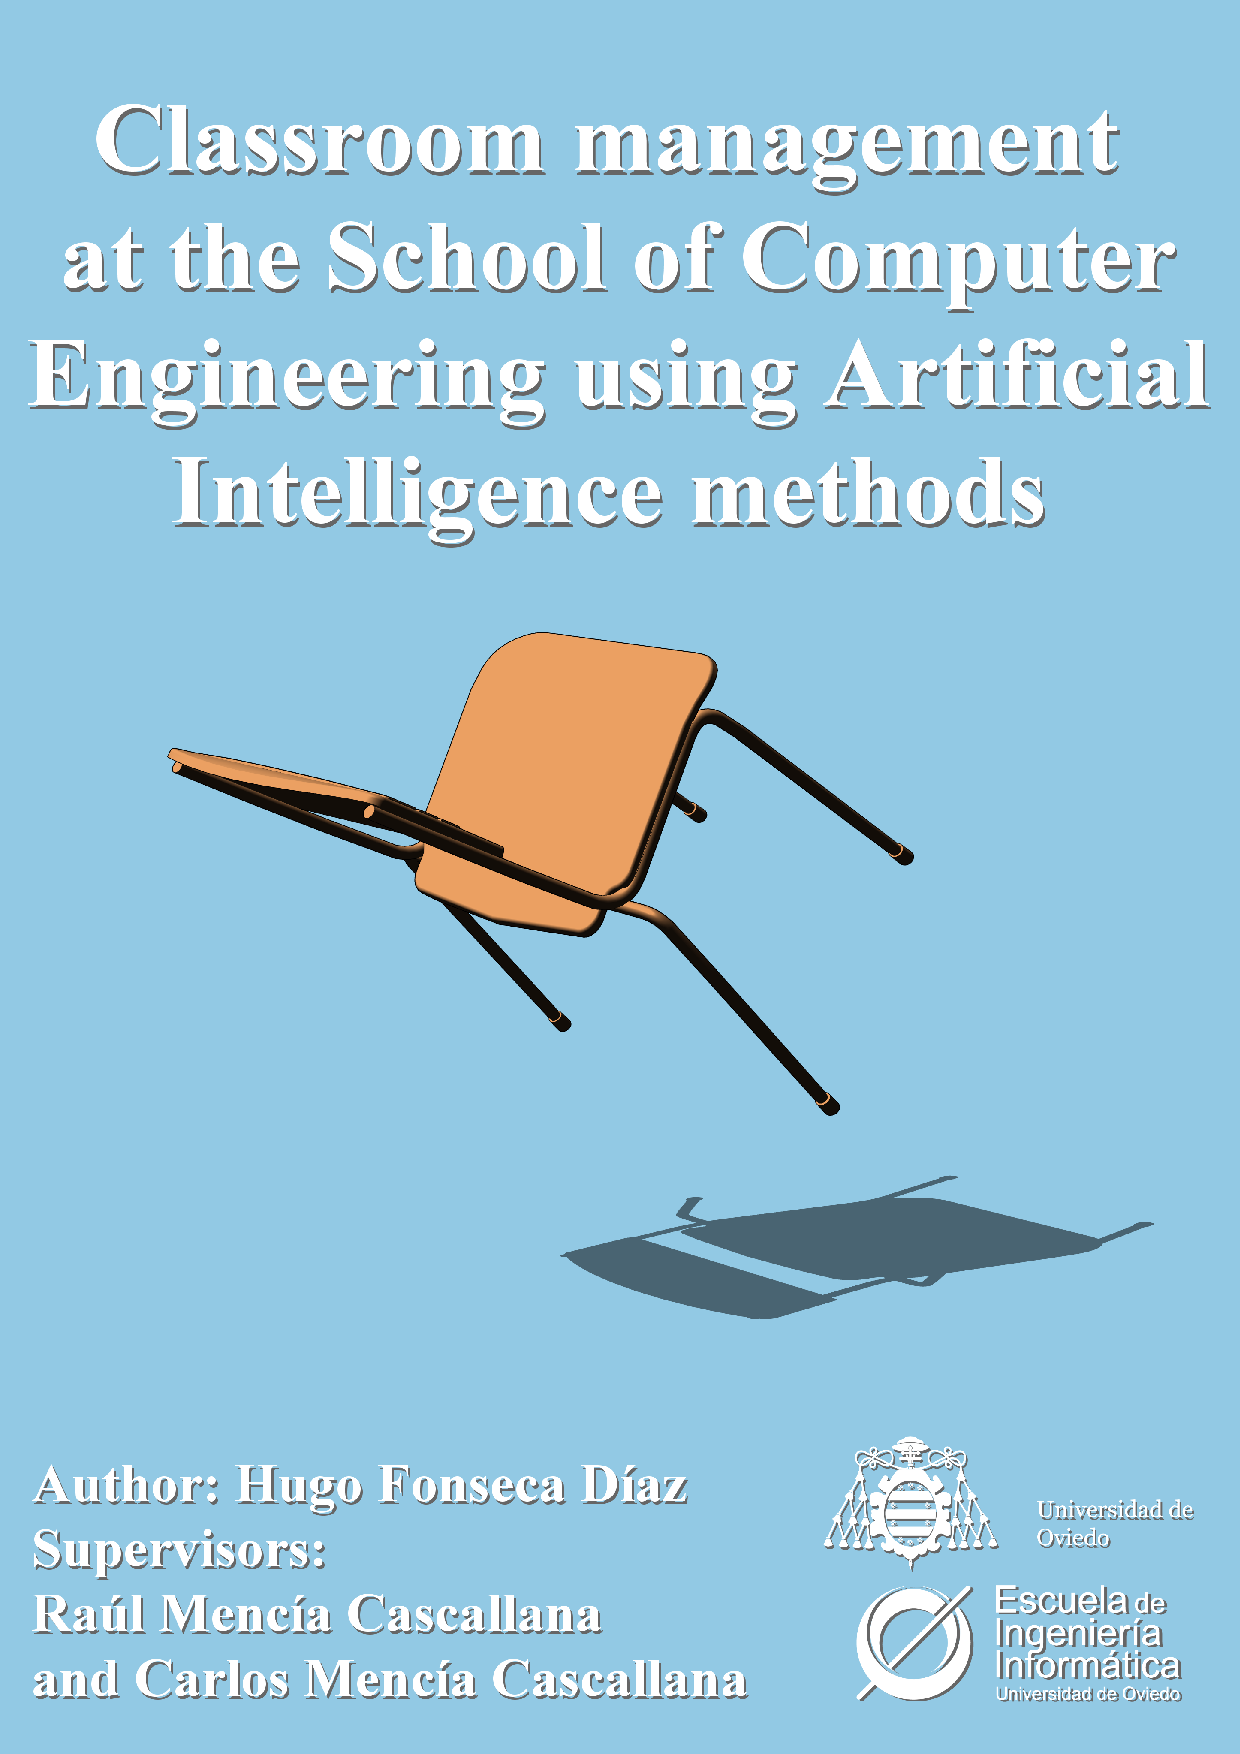
\includepdf[pages=1]{other/covers.pdf}




\renewcommand{\contentsname}{\empty}
\renewcommand{\documentname}{Index}


\chapter{Index}

\begingroup
\let\clearpage\relax

\vspace{5mm}

% Index
\tableofcontents

\endgroup


\justify % Justify text
\setlength{\parskip}{\baselineskip} % Separate paragraphs by one line
\onehalfspacing


% Content block
{
    % Links in the content block appear in blue
    \hypersetup{linkcolor=blue}

    \newpage
    \renewcommand{\documentname}{Report}

\chapter{Report}

\section{Introduction}

This document presents all the important information regarding the \tfg final degree project.

First, a report of the project is given. It functions as a general summary of the work done. The current and past situation in relation with the problem to solve are outlined, followed by briefly describing the proposed solution and the summary of the planning and budget.

Then, all the annexes are presented. They are geared towards the technical reader, and contain the initial documentation for the project, the complete system analysis and design, how the planning was elaborated, the studies related to the algorithms to be used for the implementation and finally the manuals for users and programmers of the final program.

The annexes are followed by the complete list of the requirements, functional and non-functional, and the internal and client budget breakdown.

Finally, the conclusions, future work and bibliography complete the document.

It is important to note that the organization of the contents for this document is done following the criteria and recommendations of the UNE 157801 norm for the development of information systems projects.

\section{Purpose}

This project aims to create a program that automates the process of assigning classrooms to all the groups of a given semester.

The implementation of this system is intended to assist in the work of the supervisor for this process, and provide an efficient and flexible tool that expands the possibilities of such work.

To do so, the program executes two algorithms, a genetic algorithm guided by a greedy algorithm. For a more detailed view on these algorithms the reader might refer to \ref{alg-studies}.

Along with the system, the user and programmer manuals are submitted. These have the purpose of teaching how to use, maintain and extend the system.

\section{Background}

At the beginning of each semester, the School of Computing Engineering of the University of Oviedo opens a process in which the person in charge takes the list of groups for the semester, their schedules and the list of classrooms, and performs a manual compilation of all the assignments.

There are some other similar procedures, like the creation of the exam timetable or the assignments of enrolled students to subject groups. However, some are not manual, but automated by a system, like the previously mentioned procedure of assigning students to groups.

Seeing the potential of such tool, the author of this project was given the task of automating the assignment of classrooms to subject groups. 

\section{Description of the current situation}

As explained in the previous section, the school has a supervisor for the process of assigning classrooms to groups.

This procedure is done after configuring the student groups for the semester and knowing their schedules.

Even though it is a manual process, the supervisor does not start making the assignments from scratch. First, they have the knowledge of previous years, and then they have a list of preferences or premade assignments. For example, certain laboratories can only be assigned to specific groups, like the ones from the Electronic Technology of Computers subject.

The system described in this document preserves these sources of information and builds on top of them.

\section{Standards and references}

\subsection{Standards}

\textit{UNE 157801. General criteria for the design of information systems projects.} This standard is used for defining the structure and contents of this document. However, some sections have been added, removed or modified to fit the format of a final degree project. A conclusions chapter has been introduced to the general structure as well.

\subsection{Licenses}

The software of this project is licensed under the GNU General Public License v2.0.

\subsection{Other references}

\textit{Java Code Conventions.} Set of guidelines and conventions for programmers to consider when using the Java programming language.

\section{Definitions and abbreviations}

Listed below is a glossary of definitions and abbreviations used in the document whose meaning may not be obvious.

Glossary of definitions:

\begin{itemize}
    \item \textbf{Genetic algorithm:} metaheuristic search and optimization algorithm. 
    \item \textbf{Greedy algorithm:} algorithm that builds the solution in successive steps, always trying to take the optimal solution for each step
    \item \textbf{Heuristic:} function that gives value to each path in a search algorithm, based on current information.
    \item \textbf{Java:} general-purpose, high-level, object-oriented programming language.
    \item \textbf{Metaheuristic:} high-level heuristic that guides the search in a combinatorial optimization problem.
    \item \textbf{Program:} The software described in this document.
    \item \textbf{System:} The software described in this document.
    \item \textbf{Technical reader:} used in this document as someone who knows about software engineering, but not necessarily about genetic or greedy algorithms.
\end{itemize}

Glossary of abbreviations:

\begin{itemize}
    \item \textbf{CSV:} Comma-Separated Values. Refers to a text file format.
    \item \textbf{CLI:} Command Line Interface.
    \item \textbf{GNU:} GNU is not Unix (recursive acronym). Refers to the free software project announced by Richard Stallman.
    \item \textbf{TXT:} Text. Refers to the text file format.
    \item \textbf{UNE:} in spanish, \textit{Una Norma Española}. Refers to the Spanish Association for Standardisation.
\end{itemize}

\section{Initial requirements}

The requirements listed here are a basic overview of the fundamental functionality covered by the project. For the complete list of in-depth requirements the reader might refer to \ref{requirements}.

\subsection{Interface}

\begin{itemize}
    \item The program must implement a CLI.
        \begin{itemize}
            \item The CLI must show basic or complete information to the user depending on the given option flag.
            \item The CLI must show the encountered errors to the user before terminating the execution.
            \item The CLI must have help, license and version options.
        \end{itemize}
\end{itemize}

\subsection{Input}

\begin{itemize}
    \item The progam receives as input the classrooms, groups, group schedule and the academic weeks of each group.
    \item The program might optionally receive as input a subset of assignments already performed.
    \item The program might optionally receive as input a previous complete list of assignments but without some of the classrooms/laboratories used in it.
    \item The program might optionally receive as input a previous complete list of assignments but with more or less groups.
    \item The program might optionally recieve as input a list of classroom preferences for the groups of a particular subject, given their type (theory or laboratory) and language (english or spanish).
\end{itemize}

\subsection{Configuration}

\begin{itemize}
    \item Program configuration must allow the user to control the parameters of the genetic algorithm.
    \item Program configuration must allow the user to change the version of the program.
    \item Program configuration must allow the user to specify the folder paths for the log and output files.
    \item Program configuration can change in the middle of the course.
\end{itemize}

\subsection{Algorithm}

\begin{itemize}
    \item The program must use a genetic algorithm guided by a greedy algorithm.
    \item Language group requirements:
        \begin{itemize}
            \item English groups should go to different classrooms/laboratories from the spanish groups.
        \end{itemize}
    \item Classroom requirements:
        \begin{itemize}
            \item Some initial classroom assignments can be specified before the execution of the program and they must remain the same.
            \item The program must be able to find a gap in the current list of assignments to include a (mono/multi)-(classroom/laboratory).
            \item The number of groups of the same number and course assigned to the same theory classroom must be maximised.
            \item The number of groups of the same subject assigned to the same laboratory must be maximised.
            \item In each time slot there must be a minimum number of free laboratories.
            \item Some big laboratories must be empty for emergency reasons.
            \item The program must penalise assignments where the number of students is far below the number of computers.
            \item The laboratories must have some free space defined by the user.
            \item In small laboratories (of 16 computers) there must be at least two free computers.
            \item The program must be able to handle a split in two of a laboratory group with only one professor (for emergencies).
        \end{itemize}
\end{itemize}

\section{Assumptions and restrictions}

The assumptions and constraints that directly or indirectly affect the project are listed as follows.

\begin{itemize}
    \item \textbf{Duration of the project.} The project started on January 28\textsuperscript{th}, 2022, and must be completed before July 6\textsuperscript{th}, 2022. 
    \item \textbf{Failure to find an optimal solution.} It could be the case that the genetic algorithm failed to find the optimal solution in a reasonable time. This implies a reconsideration of the constraints of the problem, or in any case a change in the evaluation of the algorithm's solutions.
    \item \textbf{Unbearable computational cost.} Related to the previous assumption, if the optimal solution requires a machine with unreasonable high specs in order to solve the problem optimally, a change in the objectives of the project could be in place.
\end{itemize}

\section{Study of alternatives and feasibility}

\subsection{Programming Language}

There were two programming languages considered for the implementation of the system, \textbf{C} and \textbf{Java}.

Considering that:

\begin{itemize}
    \item The author and only developer of the system has worked with Java throughout his university studies, but only used C in one subject and in some of his personal projects.

    \item Java is probably less efficient than C when executing the genetic and greedy algorithms.

    \item Java code is more easy to run in other systems than C code.

    \item The program is going to be executed only a few times a year.
\end{itemize}

For this reasons, even if C would be faster in execution, because the program will not be running every day, and taking into account the other two advantages, Java was the language of choice for implementing the system.

\subsection{Format of data files}

There were two file formats taken into consideration, JSON and CSV.

Bearing in mind that:

\begin{itemize}
    \item Java has no native support for processing either format.
    \item JSON is easier to manage by web services.
    \item CSV is easier to read and write from Java than JSON.
    \item CSV can be imported into a spreadsheet editor like LibreOffice Calc or Excel for its manipulation.
    \item It is preferred not to use external code libraries to avoid licensing issues.
\end{itemize}

The decision was to choose CSV as the file format for most of the input and output files of the system.

\section{Description of the proposed solution}

The software solution proposed in this document consists of a Java command line application that takes as input the CSVs of the classrooms, subjects, groups, group schedule and group academic weeks and transforms them into a CSV containing the allocation of one class for each group, as well as a TXT file with the details of the executions in a human-readable style.

This transformation is achieved by executing a genetic algorithm that generates possible solutions to the problem and a greedy algorithm that carries out the assignments and ranks the solution. At the end of the execution the solution ranked with the highest value will be returned.

Optionally, the program accepts as input the output CSV of a previous execution and also a CSV of classroom preferences for the assignments, which assists the algorithm in ranking the solutions.

Finally, there is also a configuration file that controls the parameters of the genetic algorithm, the version of the program, and the folder path for the log and output of the system.

The main advantage of the system is its great flexibility. By focusing more on the input data than on the code, it has been possible to create a tool whose functionality adapts to the CSVs built by the user.

Use cases in the middle of the semester, like adding new groups and designating their classrooms, removing laboratories due to renovation works, finding classrooms for specific courses that only last one month, finding classrooms for exams that only happen in a week, etc. are all very easy to carry out. The user just needs to change the input CSVs in the correct way and then introduce as input the output of the execution conducted at the beginning of the semester, and the program will take the current assignments into account when allocating classsrooms for these new groups.


\section{Risk analysis}
\section{Time planning}
\section{Budget summary}
\section{Prioritisation of project documents}

 

    \newpage
    \renewcommand{\documentname}{Annexes}

\chapter{Annexes}


\section{Definitions and abbreviations}

\section{Submission contents}

 

    \newpage
    \renewcommand{\documentname}{Requirements}

\chapter{Requirements}\label{requirements}

\section{Functional requirements}
\section{Non-functional requirements}

 

    \newpage
    \renewcommand{\documentname}{Budget}

\chapter{Budget} \label{section-budget}

This chapter presents the budget for the work. First the internal budget will be calculated taking into account the environment in which we work, and then the budget of the client will be prepared with the necessary items and the benefits applied.

The working time concept is reiterated. Each week has seven working days of three hours each. It is important to bear in mind this concept of working day in order to understand some sections of the budget.

\section{Internal budget}

To calculate the internal budget we must first define our situation. We are two freelancers, a junior and a senior software engineer (see Figure \ref{fig-budget-workers}).


\begin{figure}[H]
    \caption{Freelancers description}
    \label{fig-budget-workers}
  \centering
  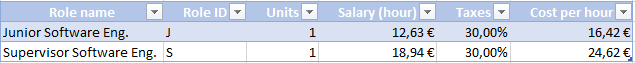
\includegraphics[scale=1]{budget_workers.PNG}
\end{figure}

We have the following rental and amortisation expenses related to the project (see Figure \ref{fig-budget-amortisations}).


\begin{figure}[H]
    \caption{Amortisation costs}
    \label{fig-budget-amortisations}
  \centering
  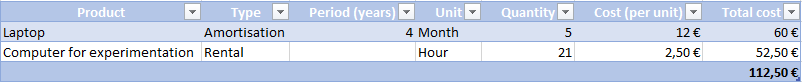
\includegraphics[scale=0.8]{budget_amortisations.PNG}
\end{figure}

Indirect costs are shown below (see Figure \ref{fig-budget-ic}).


\begin{figure}[H]
    \caption{Indirect costs}
    \label{fig-budget-ic}
  \centering
  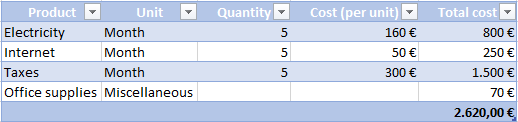
\includegraphics[scale=1]{budget_indirect_costs.PNG}
\end{figure}

Finally, we calculate the costs of carrying out the tasks defined in the WBS.


\begin{figure}[H]
    \caption{WBS Budget costs: Project Management and Analysis}
    \label{fig-budget-wbs-01}
  \centering
  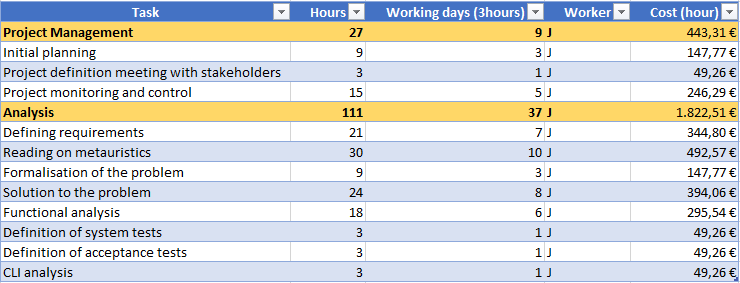
\includegraphics[scale=0.7]{budget_wbs_01.PNG}
\end{figure}


\begin{figure}[H]
    \caption{WBS Budget costs: Design and Development}
    \label{fig-budget-wbs-02}
  \centering
  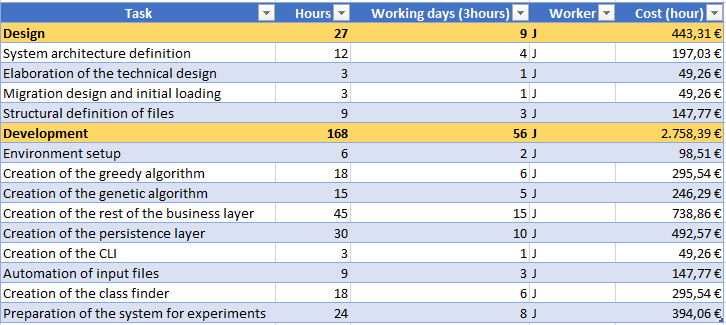
\includegraphics[scale=0.7]{budget_wbs_02.PNG}
\end{figure}


\begin{figure}[H]
    \caption{WBS Budget costs: Documentation, Experiments and Closure}
    \label{fig-budget-wbs-03}
  \centering
  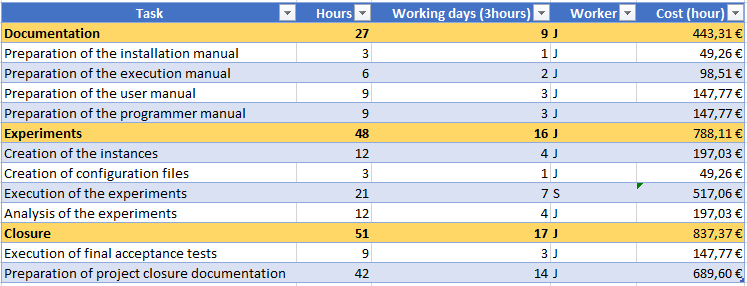
\includegraphics[scale=0.7]{budget_wbs_03.PNG}
\end{figure}

So we are left with the following cost of the WBS phases (see Figure \ref{fig-budget-wbs-sum}).


\begin{figure}[H]
    \caption{WBS Budget costs: Summary}
    \label{fig-budget-wbs-sum}
  \centering
  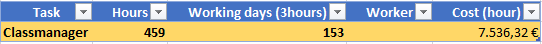
\includegraphics[scale=0.7]{budget_wbs_04.PNG}
\end{figure}

With the addition of all the costs calculated so far, we obtain the internal budget for the project.


\begin{figure}[H]
    \caption{Internal budget}
    \label{fig-budget-internal}
  \centering
  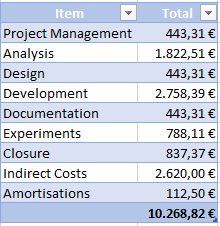
\includegraphics[scale=1]{budget_internal.PNG}
\end{figure}



\section{Client budget}


This project is expected to yield a profit of 25\%. With this information we will proceed to calculate the client's budget. It is important to note that the client will not be shown a budget with all the items, only the generic ones that describe the work to be done. Therefore, we must calculate the amount of the items not shown added to the benefits, and thus obtain a weighting value with which to calculate the client's final budget.

Figure \ref{fig-budget-weight} demonstrates the calculation of this weighting value.


\begin{figure}[H]
    \caption{Weighting value calculation}
    \label{fig-budget-weight}
  \centering
  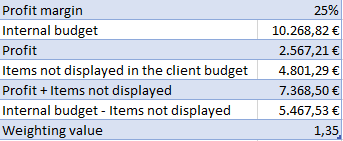
\includegraphics[scale=1]{budget_weighting.PNG}
\end{figure}

Each item is added to its own value multiplied by the weighting value and entered into the client's final budget (See Figure \ref{fig-budget-client}). This means that a cost $c_{i}$ shown in the internal budget will be transformed into a new cost if the item appears in the client budget. This transformation is given by $x_{i} = c_{i} + c_{i} w$, where $w$ is the weighting value. 


\begin{figure}[H]
    \caption{Client budget}
    \label{fig-budget-client}
  \centering
  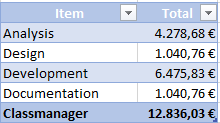
\includegraphics[scale=1]{budget_client.PNG}
\end{figure}




 

    \newpage
    \renewcommand{\documentname}{Conclusions}

\chapter{Conclusions}

\section{Future work}
\section{Final conclusions}

 

    \newpage
    \renewcommand{\documentname}{Bibliography}

\chapter{Bibliography}

\section{TODO}

TODO



}

\renewcommand{\documentname}{Bibliography}

\end{document}

